\section{Auswertung}
\label{sec:Auswertung}

Die Messungen werden für zwei Heizraten ausgeführt. Im ersten Schritt werden diese beiden Heizraten aus der Temperatur-Zeit-Abhängigkeit bestimmt. Mit einer Ausgleichsgeraden durch die gemessenen Daten, können die Heizraten bestimmt werden. Die dazugehörigen Daten sind in Abb. \ref{abb:rate} zu sehen. 

Die Werte der beiden Heizraten, die sich aus der Steigung der Ausgleichsgeraden ergeben liegen bei 
\begin{align*}
    b_1 &= \SI{1.824(9)}{\kelvin\per\minute} \\
    b_2 &= \SI{1.253(9)}{\kelvin\per\minute}. \\
\end{align*}
Die Temperaturen zur Zeit $t=\SI{0}{\second}$ sind an dieser Stelle irrelevant, werden der Vollständigkeit halber aber trotzdem angegeben mit 
\begin{align*}
    T_\text{Start, 1} &= \SI{218.68(20)}{\kelvin} \\
    T_\text{Start, 2} &= \SI{231.41(22)}{\kelvin}. \\
\end{align*}
\begin{figure}
    \centering
    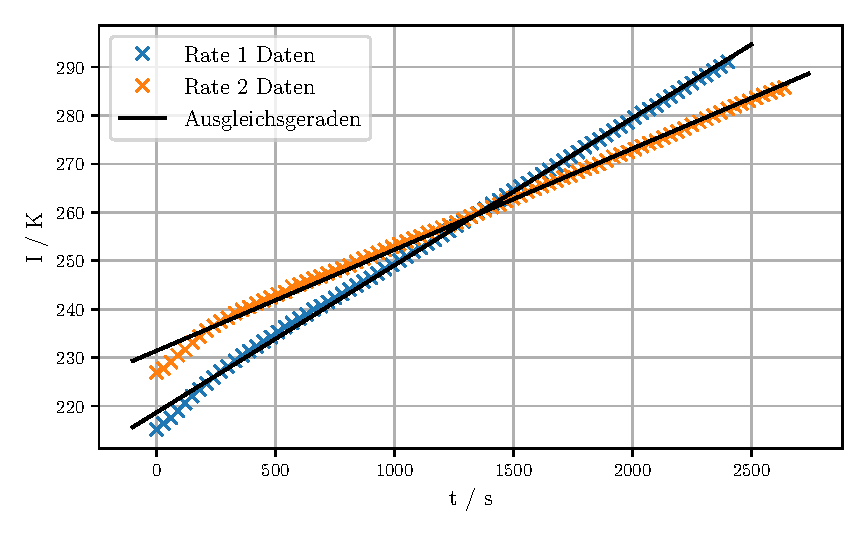
\includegraphics[width=0.8\textwidth]{figures/rate.pdf}
    \caption{Die Temperatur-Zeit-Abhängigkeit bei den jeweiligen Messungen. Es wurde alle dreißig Sekunden eine Temperatur aufgenommen. Die erste Heizrate ergibt sich zu \SI{1.824(9)}{\kelvin\per\minute}, die andere liegt bei \SI{1.253(9)}{\kelvin\per\minute}.}
    \label{abb:rate}
\end{figure}
In Abb. \ref{abb:strom1} und Abb. \ref{abb:strom2} sind die Strom-Temperaturkurven angegeben. Der gemessene Strom hat dabei die Größenordnung \num{e-12} Ampere. Zur Bereinigung des Untergrunds wird eine Exponentialfunktion der Form 
\begin{equation*}
f(T) = a \cdot \exp\left(- \frac{b}{T}\right)
\end{equation*}  
an die Werte im Bereich außerhalb des Peaks gefittet und von den gesamten Daten abgezogen. Die Fitparameter, die sich dadurch ergeben sind 
\begin{align*}
    a_{1} &= \SI{1.39(27)e-7}{\ampere} \\
    b_{1} &= \SI{2.79(6)e3}{\kelvin} \\
    a_{2} &= \SI{3.5(4)e-8}{\pico\ampere} \\
    b_{2} &= \SI{2.46(4)e3}{\kelvin}. \\
\end{align*}
\begin{figure}
    \centering
    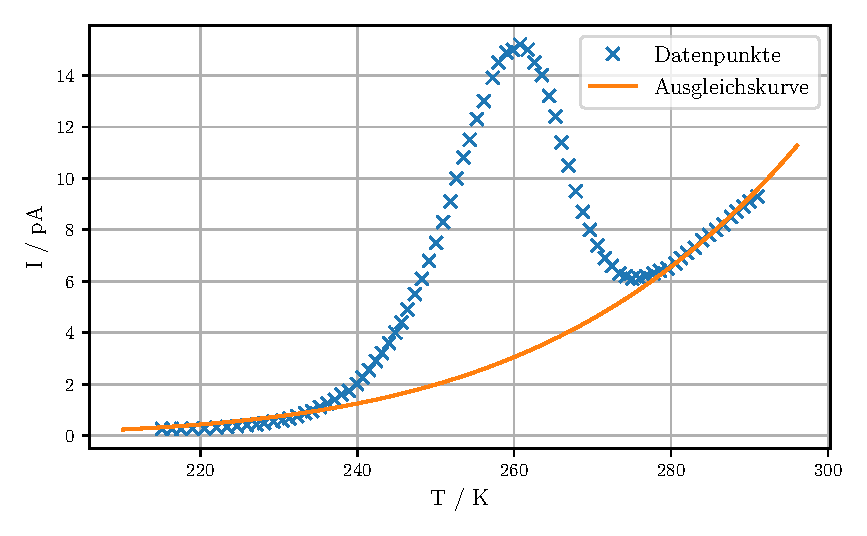
\includegraphics[width=0.6\textwidth]{figures/data_w_bkg1.pdf}
    \caption{Die gemessenen Daten der Abhängigkeit zwischen Strom und Temperatur bei Heizrate 1. Im Allgemeinen kann der Verlauf als exponentielle Kurve gefittet werden in Kombination mit z.B. einer Gauß-Kurve. Hier wurde vereinfacht nur die Exponentialfunktion gefittet.}
    \label{abb:strom1}
\end{figure}
\begin{figure}
    \centering
    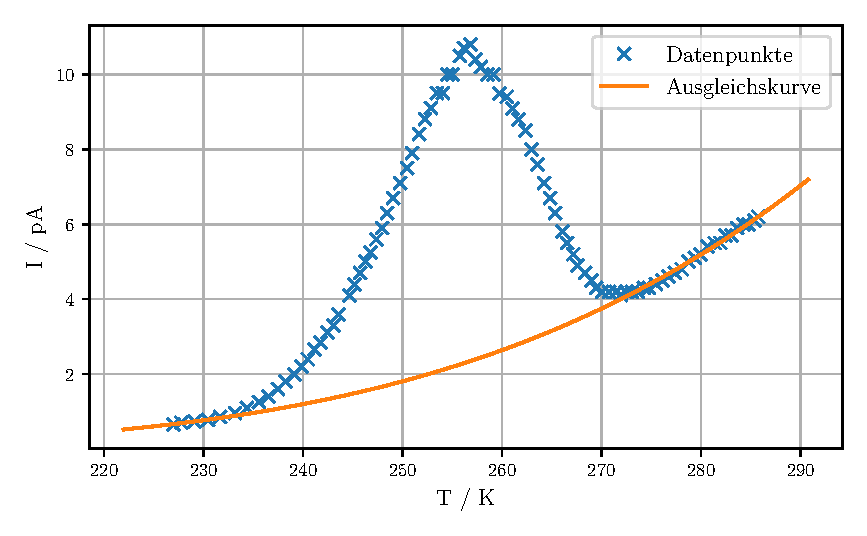
\includegraphics[width=0.6\textwidth]{figures/data_w_bkg2.pdf}
    \caption{Die gemessenen Daten der Abhängigkeit zwischen Strom und Temperatur bei Heizrate 2. Im Allgemeinen kann der Verlauf als exponentielle Kurve gefittet werden in Kombination mit z.B. einer Gauß-Kurve. Hier wurde vereinfacht nur die Exponentialfunktion gefittet.}
    \label{abb:strom2}
\end{figure}
Nach der Subtraktion des Untergrunds entstehen die beiden in Abb. \ref{abb:wo_bkg1} und Abb. \ref{abb:wo_bkg2} dargestellten Plots in denen durch die Variation der Farben erklärt ist, welche Werte für welches Verfahren im Folgenden genutzt werden. Die grünen Werte werden für die Ermittlung der Aktivierungsenergie $W$ durch die Näherung im Bereich der Anlaufkurve mit Gleichung \eqref{eq:anlauf} genutzt und der gesamte Bereich aus orangenen und grünen Datenpunkten wird für das Integral-Verfahren mit Gleichung \eqref{eq:integral} verwendet. 
\begin{figure}
    \centering
    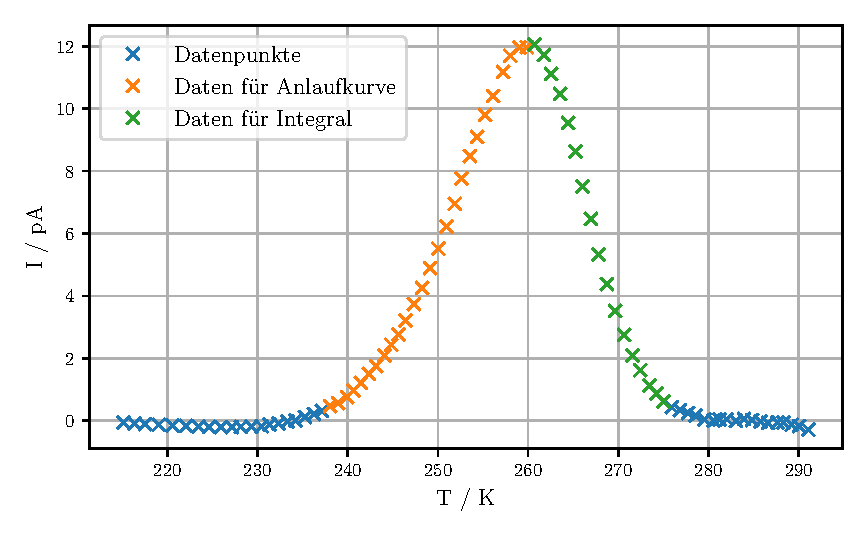
\includegraphics[width=0.6\textwidth]{figures/data_wo_bkg1.pdf}
    \caption{Die Messwerte der ersten Heizrate nachdem der gefittete Untergrund abgezogen wurde. Besonders hervorgehoben sind die Daten, die im Anschluss für die beiden Verfahren zur Bestimmung der Aktivierungsenergie $W$ benutzt werden. Die Daten für die Anlaufkurve sind in orange dargestellt, die Daten für das Integral-Verfahren sind die orangenen und die grünen Werte.}
    \label{abb:wo_bkg1}
\end{figure}
\begin{figure}
    \centering
    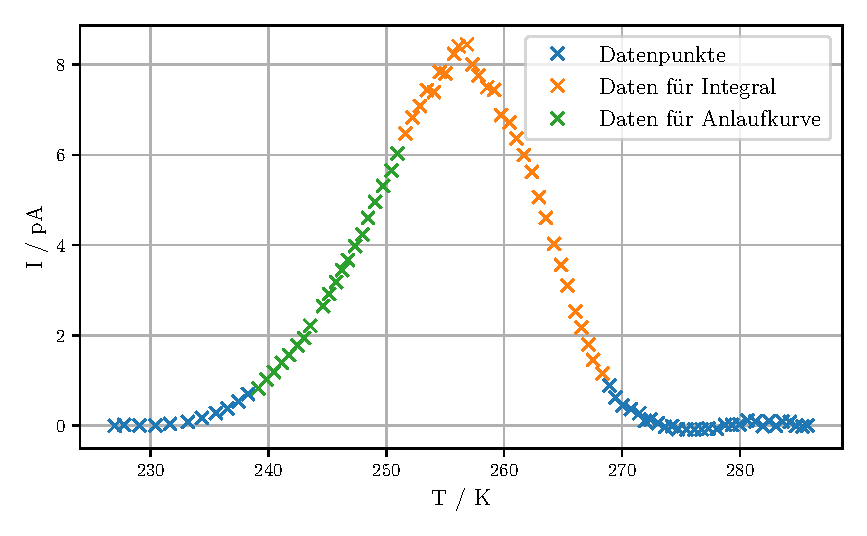
\includegraphics[width=0.6\textwidth]{figures/data_wo_bkg2.pdf}
    \caption{Die Messwerte der zweiten Heizrate nachdem der gefittete Untergrund abgezogen wurde. Besonders hervorgehoben sind die Daten, die im Anschluss für die beiden Verfahren zur Bestimmung der Aktivierungsenergie $W$ benutzt werden. Die Daten für die Anlaufkurve sind in orange dargestellt, die Daten für das Integral-Verfahren sind die orangenen und die grünen Werte.}
    \label{abb:wo_bkg2}
\end{figure}
Die orangenen Werte werden also logarithmiert und als Gerade gegen die inverse Temperatur gefittet. Der sich daraus ergebende Wert ist bereits proportional zur Aktivierungsenergie $W$, muss aber noch mit der Boltzmann Konstante multipliziert werden, damit er der Aktivierungsenergie $W$ entspricht. Die Steigung $m$ der Geraden und deren Schnittpunkt mit der $I$-Achse $n$ ergeben sich zu 
\begin{align*}
     m_{1} &= \num{-8.36(27)e3} \\
     n_{1} &= \num{35.1(11)} \\
     m_{2} &= \num{-9.87(28)e3} \\
     n_{2} &= \num{41.2(11)}. \\
\end{align*}
Somit liegen die beiden Aktivierungsenergien $W$, die sich daraus ergeben bei 
\begin{align*}
    W_{1} &= \SI{0.721(24)}{\electronvolt} \\
    W_{2} &= \SI{0.851(24)}{\electronvolt}. \\
\end{align*}
Die Werte und die Ausgleichsgeraden sind in Abb. \ref{abb:anlauf1} und Abb. \ref{abb:anlauf2} dargestellt. 

\begin{figure}
    \centering
    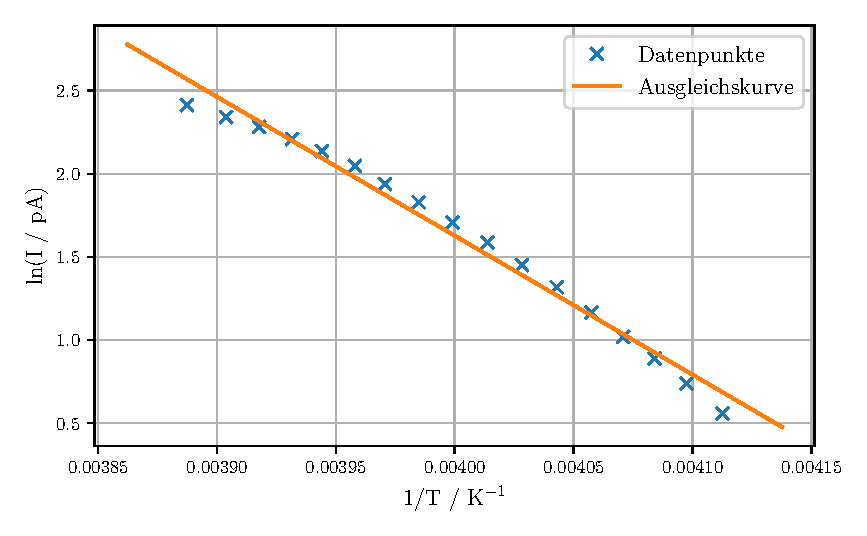
\includegraphics[width=0.7\textwidth]{figures/anlauf1.pdf}
    \caption{Die inverse Temperatur aufgetragen gegen den logarithmierten Strom der ersten Heizrate. Genähert ergibt sich daraus eine Gerade, deren Steigung proportional zur Aktivierungsenergie ist.}
    \label{abb:anlauf1}
\end{figure}

\begin{figure}
    \centering
    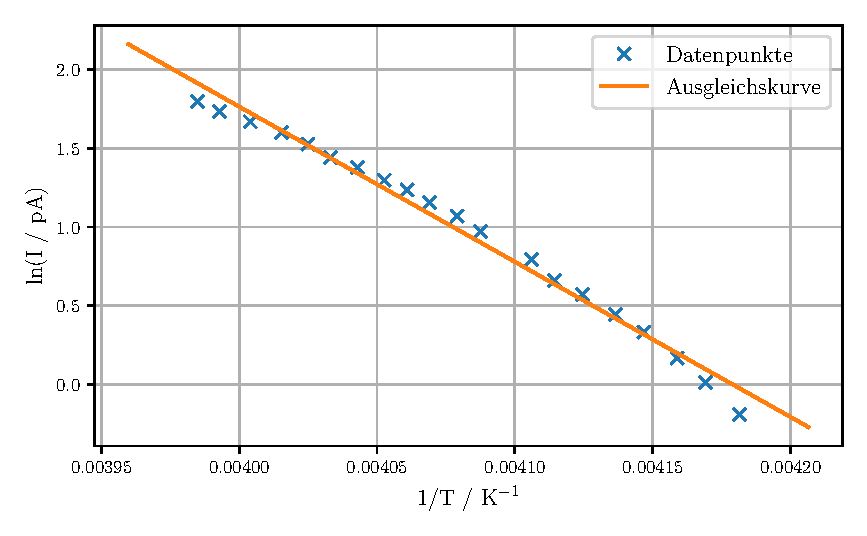
\includegraphics[width=0.7\textwidth]{figures/anlauf2.pdf}
    \caption{Die inverse Temperatur aufgetragen gegen den logarithmierten Strom der ersten Heizrate. Genähert ergibt sich daraus eine Gerade, deren Steigung proportional zur Aktivierungsenergie ist.}
    \label{abb:anlauf2}
\end{figure}

Das Integralverfahren nach Gleichung \eqref{eq:integral} wird mithilfe der Simpson Regel ausgeführt. Der Bereich der orangenen und grünen Werte wird dabei Schrittweise integriert und entsprechend der Gleichung ergibt sich dann ein linearer Zusammenhang.
Aus der ermittelten Steigung lässt sich erneut die Aktivierungsenergie $W$ bestimmen. Die Werte und Geraden sind in Abb. \ref{abb:integral1} und \ref{abb:integral2} dargestellt. Die Werte die sich durch die Ausgleichsrechnung ergeben, sind 
\begin{align*}
    m_{1} &= \num{1.011(17)e4} \\
    n_{1} &= \num{-37.5(7)} \\
    m_{2} &= \num{1.049(16)e4} \\
    n_{2} &= \num{-39.1(6)} \\
\end{align*}
und die beiden Aktivierungsenergien $W$, die sich daraus ergeben sind 
\begin{align*}
    W_{1} &= \SI{0.871(15)}{\electronvolt} \\
    W_{2} &= \SI{0.904(14)}{\electronvolt}. \\
\end{align*}

\begin{figure}
    \centering
    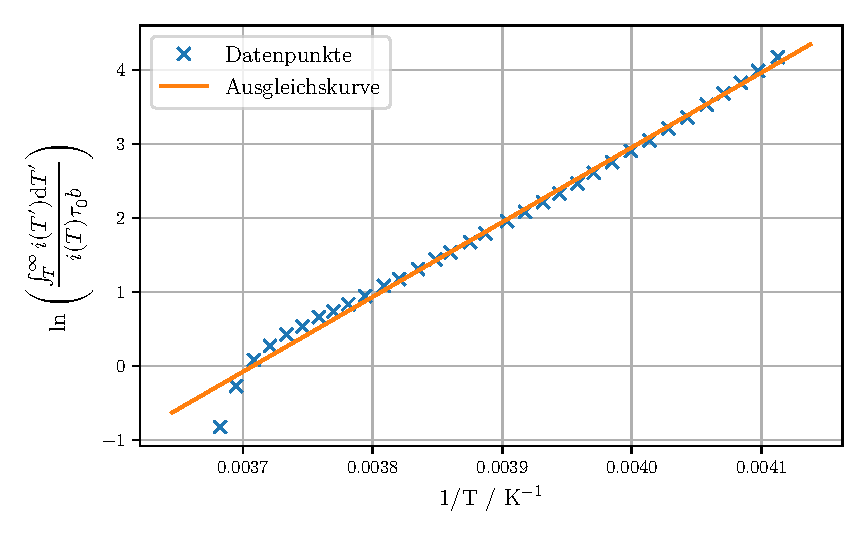
\includegraphics[width=0.7\textwidth]{figures/integral1.pdf}
    \caption{Die inverse Temperatur aufgetragen gegen den logarithmierten integrierten Strom dividiert durch den Strom und die erste Heizrate. Genähert ergibt sich daraus eine Gerade, deren Steigung proportional zur Aktivierungsenergie ist.}
    \label{abb:integral1}
\end{figure}

\begin{figure}
    \centering
    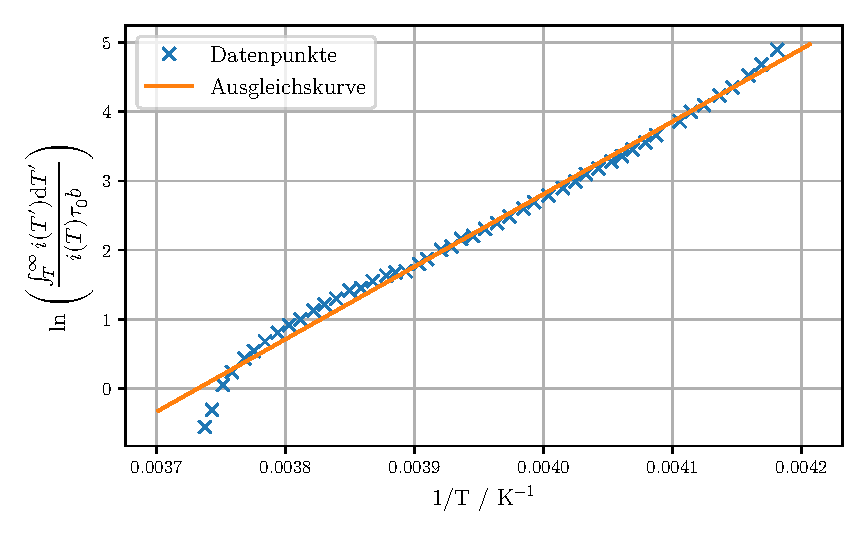
\includegraphics[width=0.7\textwidth]{figures/integral2.pdf}
    \caption{Die inverse Temperatur aufgetragen gegen den logarithmierten integrierten Strom dividiert durch den Strom und die erste Heizrate. Genähert ergibt sich daraus eine Gerade, deren Steigung proportional zur Aktivierungsenergie ist.}
    \label{abb:integral2}
\end{figure}

Mithilfe der ermittelten Aktivierungsenergie $W$ ergibt sich über Gleichung \eqref{eq:tmax} und die Temperaturen bei den Maxima der Kurven, die bei 
\begin{align*}
    T_\text{max,1} &= \SI{260.75}{\kelvin} \\
    T_\text{max,1} &= \SI{256.85}{\kelvin} \\
\end{align*}
liegen, die Zeit $\tau_0$ für beide Heizraten. Da vier relativ verschiedene Werte für die Aktivierungsenergien $W$ bestimmt wurden, ergeben sich daraus auch vier verschiedene Werte für $\tau_0$.
Diese sind 
\begin{align*}
    \tau_\text{0, 1, Anlauf} &= \SI{5(6)e-14}{\second} \\
    \tau_\text{0, 1, Integral} &= \SI{5(4)e-17}{\second} \\
    \tau_\text{0, 2, Anlauf} &= \SI{1.1(12)e-16}{\second} \\
    \tau_\text{0, 2, Integral} &= \SI{9(6)e-18}{\second}. \\
\end{align*}

Die aus den Zeiten $\tau_0$ resultierenden Kurven nach Gleichung \eqref{eq:relax} sind in Abb. \ref{abb:tau} dargestellt.

\begin{figure}
    \centering
    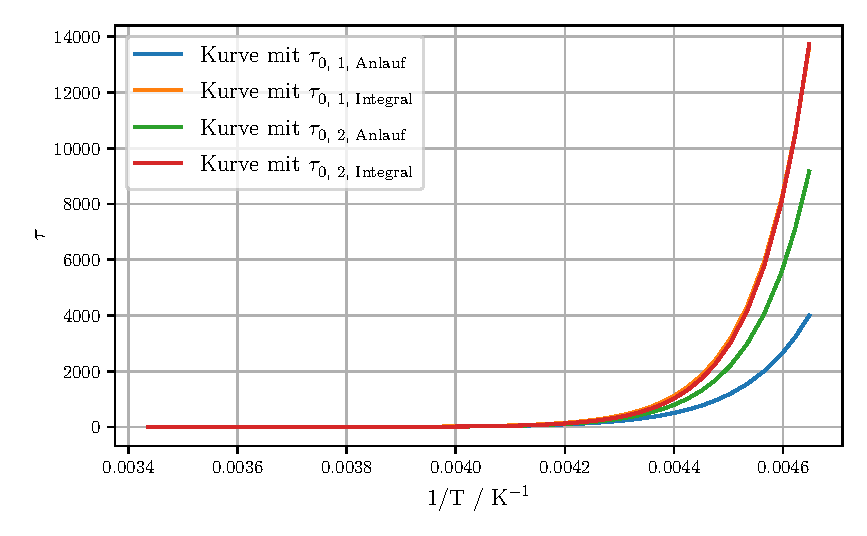
\includegraphics[width=0.7\textwidth]{figures/tau.pdf}
    \caption{Die inverse Temperatur aufgetragen gegen die temperaturabhängige Relaxationszeit nach Gleichung \eqref{eq:relax}. Die Kurve wurde für die vier verschiedenen Werte von der charakteristischen Relaxationszeit $\tau_0$ und der dazugehörigen Aktivierungsenergie $W$ bestimmt. Die Kurven der beiden durch das Integral-Verfahren ermittelten Werte sieht beinahe identisch aus.}
    \label{abb:tau}
\end{figure}

